% ---------------------------------------------------------------
%  EnergyTech / معهد الطاقة  --  Chapter 04, version D
%  Questions + answer choices + QR codes.
%  Scale diagrams are TikZ; the two labelled instrument photographs
%  live in figures/.
%  Compile with pdflatex (needs the 'qrcode' package).
% ---------------------------------------------------------------
\documentclass[11pt]{article}
\usepackage[a4paper,margin=1.8cm]{geometry}
\usepackage{amsmath,amssymb}
\usepackage{enumitem}
\usepackage{qrcode}
\usepackage{graphicx}
\usepackage{xcolor}
\usepackage[hidelinks]{hyperref}
\usepackage{multicol}

\setlength{\parindent}{0pt}
\setlength{\columnsep}{20pt}
\graphicspath{{figures/}}

\newcommand{\incfig}[2]{%
  \par\smallskip\begingroup\centering
  \ifdim #1pt>\linewidth\relax
    \includegraphics[width=\linewidth]{#2}%
  \else
    \includegraphics[width=#1pt]{#2}%
  \fi
  \par\endgroup\smallskip}

\newenvironment{Qbox}[2]{%
  \par\medskip\noindent\begin{minipage}{\linewidth}%
  \hrule\medskip%
  \textbf{Q#1)}\hfill\textbf{\underline{#2}}\par\smallskip%
}{\par\end{minipage}\par\medskip}

\newlist{choices}{enumerate}{1}
\setlist[choices]{label=\Alph*), itemsep=1pt, topsep=3pt, parsep=0pt, leftmargin=2em}
% ---------------------------------------------------------------

% ================= figure styles =================
\usepackage{tikz}
\usetikzlibrary{arrows.meta,calc,shadings}

\definecolor{figline}{RGB}{30,30,30}
\definecolor{figpanel}{RGB}{243,243,243}
\definecolor{figmark}{RGB}{63,63,160}
\definecolor{figbody}{RGB}{232,234,238}
\definecolor{figthimble}{RGB}{205,210,219}

\tikzset{
  sc/.style   ={draw=figline, line width=0.5pt, line cap=butt},
  scb/.style  ={draw=figline, line width=0.8pt},
  lab/.style  ={font=\small\bfseries, inner sep=1pt},
  labs/.style ={font=\scriptsize\bfseries, inner sep=1pt},
  ptr/.style ={draw=figmark, line width=1pt, -{Latex[length=4pt,width=3.5pt]}},
}

\newcommand{\figbox}[1]{%
  \par\smallskip\begingroup\centering
  \sbox0{#1}%
  \ifdim\wd0>\linewidth \resizebox{\linewidth}{!}{\usebox0}\else\usebox0\fi
  \par\endgroup\smallskip}

% ---- figure definitions ----
\newcommand{\figQBZ}{%
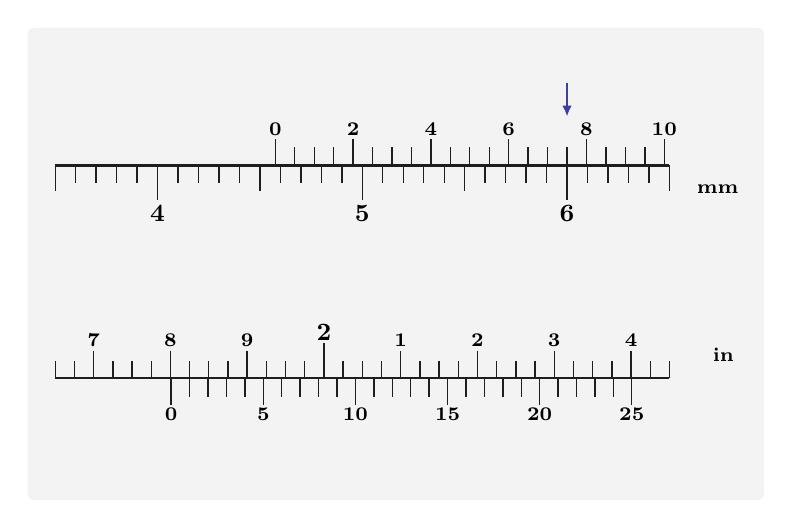
\begin{tikzpicture}[scale=1]
  \fill[figpanel,rounded corners=2pt] (-0.35,-1.55) rectangle (9,4.45);
  \begin{scope}[yshift=2.70cm]
  \draw[scb] (0,0) -- (7.8,0);
  \draw[sc] (0,0) -- (0,-0.32);
  \draw[sc] (0.26,0) -- (0.26,-0.22);
  \draw[sc] (0.52,0) -- (0.52,-0.22);
  \draw[sc] (0.78,0) -- (0.78,-0.22);
  \draw[sc] (1.04,0) -- (1.04,-0.22);
  \draw[sc] (1.3,0) -- (1.3,-0.44);
  \node[lab,below] at (1.3,-0.46) {4};
  \draw[sc] (1.56,0) -- (1.56,-0.22);
  \draw[sc] (1.82,0) -- (1.82,-0.22);
  \draw[sc] (2.08,0) -- (2.08,-0.22);
  \draw[sc] (2.34,0) -- (2.34,-0.22);
  \draw[sc] (2.6,0) -- (2.6,-0.32);
  \draw[sc] (2.86,0) -- (2.86,-0.22);
  \draw[sc] (3.12,0) -- (3.12,-0.22);
  \draw[sc] (3.38,0) -- (3.38,-0.22);
  \draw[sc] (3.64,0) -- (3.64,-0.22);
  \draw[sc] (3.9,0) -- (3.9,-0.44);
  \node[lab,below] at (3.9,-0.46) {5};
  \draw[sc] (4.16,0) -- (4.16,-0.22);
  \draw[sc] (4.42,0) -- (4.42,-0.22);
  \draw[sc] (4.68,0) -- (4.68,-0.22);
  \draw[sc] (4.94,0) -- (4.94,-0.22);
  \draw[sc] (5.2,0) -- (5.2,-0.32);
  \draw[sc] (5.46,0) -- (5.46,-0.22);
  \draw[sc] (5.72,0) -- (5.72,-0.22);
  \draw[sc] (5.98,0) -- (5.98,-0.22);
  \draw[sc] (6.24,0) -- (6.24,-0.22);
  \draw[sc] (6.5,0) -- (6.5,-0.44);
  \node[lab,below] at (6.5,-0.46) {6};
  \draw[sc] (6.76,0) -- (6.76,-0.22);
  \draw[sc] (7.02,0) -- (7.02,-0.22);
  \draw[sc] (7.28,0) -- (7.28,-0.22);
  \draw[sc] (7.54,0) -- (7.54,-0.22);
  \draw[sc] (7.8,0) -- (7.8,-0.32);
  \draw[sc] (2.795,0) -- (2.795,0.34);
  \node[labs,above] at (2.795,0.34) {0};
  \draw[sc] (3.042,0) -- (3.042,0.24);
  \draw[sc] (3.289,0) -- (3.289,0.24);
  \draw[sc] (3.536,0) -- (3.536,0.24);
  \draw[sc] (3.783,0) -- (3.783,0.34);
  \node[labs,above] at (3.783,0.34) {2};
  \draw[sc] (4.03,0) -- (4.03,0.24);
  \draw[sc] (4.277,0) -- (4.277,0.24);
  \draw[sc] (4.524,0) -- (4.524,0.24);
  \draw[sc] (4.771,0) -- (4.771,0.34);
  \node[labs,above] at (4.771,0.34) {4};
  \draw[sc] (5.018,0) -- (5.018,0.24);
  \draw[sc] (5.265,0) -- (5.265,0.24);
  \draw[sc] (5.512,0) -- (5.512,0.24);
  \draw[sc] (5.759,0) -- (5.759,0.34);
  \node[labs,above] at (5.759,0.34) {6};
  \draw[sc] (6.006,0) -- (6.006,0.24);
  \draw[sc] (6.253,0) -- (6.253,0.24);
  \draw[sc] (6.5,0) -- (6.5,0.24);
  \draw[sc] (6.747,0) -- (6.747,0.34);
  \node[labs,above] at (6.747,0.34) {8};
  \draw[sc] (6.994,0) -- (6.994,0.24);
  \draw[sc] (7.241,0) -- (7.241,0.24);
  \draw[sc] (7.488,0) -- (7.488,0.24);
  \draw[sc] (7.735,0) -- (7.735,0.34);
  \node[labs,above] at (7.735,0.34) {10};
  \draw[ptr] (6.5,1.05) -- (6.5,0.62);
  \node[labs,left] at (8.72,-0.30) {mm};
  \end{scope}
  \begin{scope}[yshift=0cm]
  \draw[scb] (0,0) -- (7.8,0);
  \draw[sc] (0,0) -- (0,0.22);
  \draw[sc] (0.2438,0) -- (0.2438,0.22);
  \draw[sc] (0.4875,0) -- (0.4875,0.34);
  \node[labs,above] at (0.4875,0.36) {7};
  \draw[sc] (0.7313,0) -- (0.7313,0.22);
  \draw[sc] (0.975,0) -- (0.975,0.22);
  \draw[sc] (1.2188,0) -- (1.2188,0.22);
  \draw[sc] (1.4625,0) -- (1.4625,0.34);
  \node[labs,above] at (1.4625,0.36) {8};
  \draw[sc] (1.7063,0) -- (1.7063,0.22);
  \draw[sc] (1.95,0) -- (1.95,0.22);
  \draw[sc] (2.1938,0) -- (2.1938,0.22);
  \draw[sc] (2.4375,0) -- (2.4375,0.34);
  \node[labs,above] at (2.4375,0.36) {9};
  \draw[sc] (2.6813,0) -- (2.6813,0.22);
  \draw[sc] (2.925,0) -- (2.925,0.22);
  \draw[sc] (3.1688,0) -- (3.1688,0.22);
  \draw[sc] (3.4125,0) -- (3.4125,0.44);
  \node[lab,above] at (3.4125,0.44) {2};
  \draw[sc] (3.6562,0) -- (3.6562,0.22);
  \draw[sc] (3.9,0) -- (3.9,0.22);
  \draw[sc] (4.1438,0) -- (4.1438,0.22);
  \draw[sc] (4.3875,0) -- (4.3875,0.34);
  \node[labs,above] at (4.3875,0.36) {1};
  \draw[sc] (4.6313,0) -- (4.6313,0.22);
  \draw[sc] (4.875,0) -- (4.875,0.22);
  \draw[sc] (5.1188,0) -- (5.1188,0.22);
  \draw[sc] (5.3625,0) -- (5.3625,0.34);
  \node[labs,above] at (5.3625,0.36) {2};
  \draw[sc] (5.6063,0) -- (5.6063,0.22);
  \draw[sc] (5.85,0) -- (5.85,0.22);
  \draw[sc] (6.0938,0) -- (6.0938,0.22);
  \draw[sc] (6.3375,0) -- (6.3375,0.34);
  \node[labs,above] at (6.3375,0.36) {3};
  \draw[sc] (6.5813,0) -- (6.5813,0.22);
  \draw[sc] (6.825,0) -- (6.825,0.22);
  \draw[sc] (7.0688,0) -- (7.0688,0.22);
  \draw[sc] (7.3125,0) -- (7.3125,0.34);
  \node[labs,above] at (7.3125,0.36) {4};
  \draw[sc] (7.5563,0) -- (7.5563,0.22);
  \draw[sc] (7.8,0) -- (7.8,0.22);
  \draw[sc] (1.4723,0) -- (1.4723,-0.34);
  \node[labs,below] at (1.4723,-0.34) {0};
  \draw[sc] (1.7063,0) -- (1.7063,-0.24);
  \draw[sc] (1.9403,0) -- (1.9403,-0.24);
  \draw[sc] (2.1743,0) -- (2.1743,-0.24);
  \draw[sc] (2.4083,0) -- (2.4083,-0.24);
  \draw[sc] (2.6422,0) -- (2.6422,-0.34);
  \node[labs,below] at (2.6422,-0.34) {5};
  \draw[sc] (2.8762,0) -- (2.8762,-0.24);
  \draw[sc] (3.1102,0) -- (3.1102,-0.24);
  \draw[sc] (3.3442,0) -- (3.3442,-0.24);
  \draw[sc] (3.5782,0) -- (3.5782,-0.24);
  \draw[sc] (3.8123,0) -- (3.8123,-0.34);
  \node[labs,below] at (3.8123,-0.34) {10};
  \draw[sc] (4.0463,0) -- (4.0463,-0.24);
  \draw[sc] (4.2803,0) -- (4.2803,-0.24);
  \draw[sc] (4.5143,0) -- (4.5143,-0.24);
  \draw[sc] (4.7483,0) -- (4.7483,-0.24);
  \draw[sc] (4.9823,0) -- (4.9823,-0.34);
  \node[labs,below] at (4.9823,-0.34) {15};
  \draw[sc] (5.2163,0) -- (5.2163,-0.24);
  \draw[sc] (5.4503,0) -- (5.4503,-0.24);
  \draw[sc] (5.6843,0) -- (5.6843,-0.24);
  \draw[sc] (5.9183,0) -- (5.9183,-0.24);
  \draw[sc] (6.1522,0) -- (6.1522,-0.34);
  \node[labs,below] at (6.1522,-0.34) {20};
  \draw[sc] (6.3862,0) -- (6.3862,-0.24);
  \draw[sc] (6.6202,0) -- (6.6202,-0.24);
  \draw[sc] (6.8542,0) -- (6.8542,-0.24);
  \draw[sc] (7.0882,0) -- (7.0882,-0.24);
  \draw[sc] (7.3222,0) -- (7.3222,-0.34);
  \node[labs,below] at (7.3222,-0.34) {25};
  \node[labs,left] at (8.66,0.30) {in};
  \end{scope}
\end{tikzpicture}
}

\newcommand{\figQBA}{%
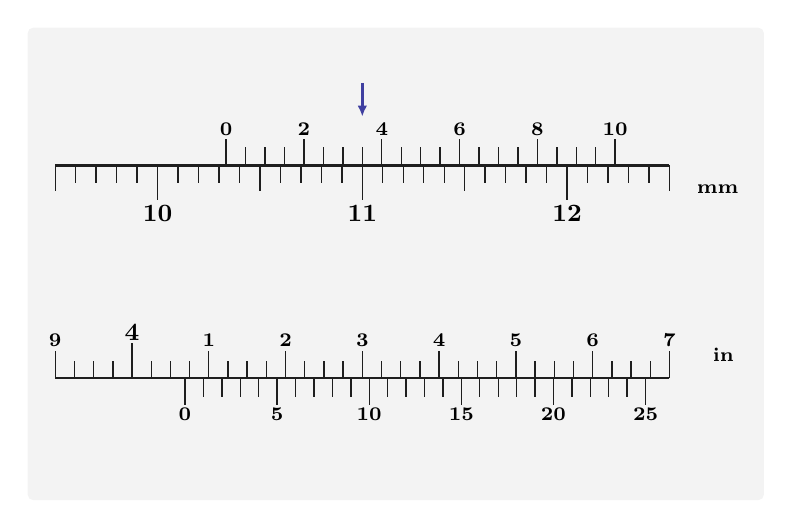
\begin{tikzpicture}[scale=1]
  \fill[figpanel,rounded corners=2pt] (-0.35,-1.55) rectangle (9,4.45);
  \begin{scope}[yshift=2.70cm]
  \draw[scb] (0,0) -- (7.8,0);
  \draw[sc] (0,0) -- (0,-0.32);
  \draw[sc] (0.26,0) -- (0.26,-0.22);
  \draw[sc] (0.52,0) -- (0.52,-0.22);
  \draw[sc] (0.78,0) -- (0.78,-0.22);
  \draw[sc] (1.04,0) -- (1.04,-0.22);
  \draw[sc] (1.3,0) -- (1.3,-0.44);
  \node[lab,below] at (1.3,-0.46) {10};
  \draw[sc] (1.56,0) -- (1.56,-0.22);
  \draw[sc] (1.82,0) -- (1.82,-0.22);
  \draw[sc] (2.08,0) -- (2.08,-0.22);
  \draw[sc] (2.34,0) -- (2.34,-0.22);
  \draw[sc] (2.6,0) -- (2.6,-0.32);
  \draw[sc] (2.86,0) -- (2.86,-0.22);
  \draw[sc] (3.12,0) -- (3.12,-0.22);
  \draw[sc] (3.38,0) -- (3.38,-0.22);
  \draw[sc] (3.64,0) -- (3.64,-0.22);
  \draw[sc] (3.9,0) -- (3.9,-0.44);
  \node[lab,below] at (3.9,-0.46) {11};
  \draw[sc] (4.16,0) -- (4.16,-0.22);
  \draw[sc] (4.42,0) -- (4.42,-0.22);
  \draw[sc] (4.68,0) -- (4.68,-0.22);
  \draw[sc] (4.94,0) -- (4.94,-0.22);
  \draw[sc] (5.2,0) -- (5.2,-0.32);
  \draw[sc] (5.46,0) -- (5.46,-0.22);
  \draw[sc] (5.72,0) -- (5.72,-0.22);
  \draw[sc] (5.98,0) -- (5.98,-0.22);
  \draw[sc] (6.24,0) -- (6.24,-0.22);
  \draw[sc] (6.5,0) -- (6.5,-0.44);
  \node[lab,below] at (6.5,-0.46) {12};
  \draw[sc] (6.76,0) -- (6.76,-0.22);
  \draw[sc] (7.02,0) -- (7.02,-0.22);
  \draw[sc] (7.28,0) -- (7.28,-0.22);
  \draw[sc] (7.54,0) -- (7.54,-0.22);
  \draw[sc] (7.8,0) -- (7.8,-0.32);
  \draw[sc] (2.171,0) -- (2.171,0.34);
  \node[labs,above] at (2.171,0.34) {0};
  \draw[sc] (2.418,0) -- (2.418,0.24);
  \draw[sc] (2.665,0) -- (2.665,0.24);
  \draw[sc] (2.912,0) -- (2.912,0.24);
  \draw[sc] (3.159,0) -- (3.159,0.34);
  \node[labs,above] at (3.159,0.34) {2};
  \draw[sc] (3.406,0) -- (3.406,0.24);
  \draw[sc] (3.653,0) -- (3.653,0.24);
  \draw[sc] (3.9,0) -- (3.9,0.24);
  \draw[sc] (4.147,0) -- (4.147,0.34);
  \node[labs,above] at (4.147,0.34) {4};
  \draw[sc] (4.394,0) -- (4.394,0.24);
  \draw[sc] (4.641,0) -- (4.641,0.24);
  \draw[sc] (4.888,0) -- (4.888,0.24);
  \draw[sc] (5.135,0) -- (5.135,0.34);
  \node[labs,above] at (5.135,0.34) {6};
  \draw[sc] (5.382,0) -- (5.382,0.24);
  \draw[sc] (5.629,0) -- (5.629,0.24);
  \draw[sc] (5.876,0) -- (5.876,0.24);
  \draw[sc] (6.123,0) -- (6.123,0.34);
  \node[labs,above] at (6.123,0.34) {8};
  \draw[sc] (6.37,0) -- (6.37,0.24);
  \draw[sc] (6.617,0) -- (6.617,0.24);
  \draw[sc] (6.864,0) -- (6.864,0.24);
  \draw[sc] (7.111,0) -- (7.111,0.34);
  \node[labs,above] at (7.111,0.34) {10};
  \draw[ptr] (3.9,1.05) -- (3.9,0.62);
  \node[labs,left] at (8.72,-0.30) {mm};
  \end{scope}
  \begin{scope}[yshift=0cm]
  \draw[scb] (0,0) -- (7.8,0);
  \draw[sc] (0,0) -- (0,0.34);
  \node[labs,above] at (0,0.36) {9};
  \draw[sc] (0.2438,0) -- (0.2438,0.22);
  \draw[sc] (0.4875,0) -- (0.4875,0.22);
  \draw[sc] (0.7313,0) -- (0.7313,0.22);
  \draw[sc] (0.975,0) -- (0.975,0.44);
  \node[lab,above] at (0.975,0.44) {4};
  \draw[sc] (1.2188,0) -- (1.2188,0.22);
  \draw[sc] (1.4625,0) -- (1.4625,0.22);
  \draw[sc] (1.7063,0) -- (1.7063,0.22);
  \draw[sc] (1.95,0) -- (1.95,0.34);
  \node[labs,above] at (1.95,0.36) {1};
  \draw[sc] (2.1938,0) -- (2.1938,0.22);
  \draw[sc] (2.4375,0) -- (2.4375,0.22);
  \draw[sc] (2.6812,0) -- (2.6812,0.22);
  \draw[sc] (2.925,0) -- (2.925,0.34);
  \node[labs,above] at (2.925,0.36) {2};
  \draw[sc] (3.1688,0) -- (3.1688,0.22);
  \draw[sc] (3.4125,0) -- (3.4125,0.22);
  \draw[sc] (3.6563,0) -- (3.6563,0.22);
  \draw[sc] (3.9,0) -- (3.9,0.34);
  \node[labs,above] at (3.9,0.36) {3};
  \draw[sc] (4.1438,0) -- (4.1438,0.22);
  \draw[sc] (4.3875,0) -- (4.3875,0.22);
  \draw[sc] (4.6313,0) -- (4.6313,0.22);
  \draw[sc] (4.875,0) -- (4.875,0.34);
  \node[labs,above] at (4.875,0.36) {4};
  \draw[sc] (5.1187,0) -- (5.1187,0.22);
  \draw[sc] (5.3625,0) -- (5.3625,0.22);
  \draw[sc] (5.6063,0) -- (5.6063,0.22);
  \draw[sc] (5.85,0) -- (5.85,0.34);
  \node[labs,above] at (5.85,0.36) {5};
  \draw[sc] (6.0938,0) -- (6.0938,0.22);
  \draw[sc] (6.3375,0) -- (6.3375,0.22);
  \draw[sc] (6.5813,0) -- (6.5813,0.22);
  \draw[sc] (6.825,0) -- (6.825,0.34);
  \node[labs,above] at (6.825,0.36) {6};
  \draw[sc] (7.0688,0) -- (7.0688,0.22);
  \draw[sc] (7.3125,0) -- (7.3125,0.22);
  \draw[sc] (7.5562,0) -- (7.5562,0.22);
  \draw[sc] (7.8,0) -- (7.8,0.34);
  \node[labs,above] at (7.8,0.36) {7};
  \draw[sc] (1.6478,0) -- (1.6478,-0.34);
  \node[labs,below] at (1.6478,-0.34) {0};
  \draw[sc] (1.8818,0) -- (1.8818,-0.24);
  \draw[sc] (2.1158,0) -- (2.1158,-0.24);
  \draw[sc] (2.3498,0) -- (2.3498,-0.24);
  \draw[sc] (2.5838,0) -- (2.5838,-0.24);
  \draw[sc] (2.8178,0) -- (2.8178,-0.34);
  \node[labs,below] at (2.8178,-0.34) {5};
  \draw[sc] (3.0518,0) -- (3.0518,-0.24);
  \draw[sc] (3.2858,0) -- (3.2858,-0.24);
  \draw[sc] (3.5198,0) -- (3.5198,-0.24);
  \draw[sc] (3.7538,0) -- (3.7538,-0.24);
  \draw[sc] (3.9878,0) -- (3.9878,-0.34);
  \node[labs,below] at (3.9878,-0.34) {10};
  \draw[sc] (4.2218,0) -- (4.2218,-0.24);
  \draw[sc] (4.4558,0) -- (4.4558,-0.24);
  \draw[sc] (4.6898,0) -- (4.6898,-0.24);
  \draw[sc] (4.9238,0) -- (4.9238,-0.24);
  \draw[sc] (5.1578,0) -- (5.1578,-0.34);
  \node[labs,below] at (5.1578,-0.34) {15};
  \draw[sc] (5.3918,0) -- (5.3918,-0.24);
  \draw[sc] (5.6258,0) -- (5.6258,-0.24);
  \draw[sc] (5.8598,0) -- (5.8598,-0.24);
  \draw[sc] (6.0938,0) -- (6.0938,-0.24);
  \draw[sc] (6.3277,0) -- (6.3277,-0.34);
  \node[labs,below] at (6.3277,-0.34) {20};
  \draw[sc] (6.5618,0) -- (6.5618,-0.24);
  \draw[sc] (6.7957,0) -- (6.7957,-0.24);
  \draw[sc] (7.0298,0) -- (7.0298,-0.24);
  \draw[sc] (7.2637,0) -- (7.2637,-0.24);
  \draw[sc] (7.4977,0) -- (7.4977,-0.34);
  \node[labs,below] at (7.4977,-0.34) {25};
  \node[labs,left] at (8.66,0.30) {in};
  \end{scope}
\end{tikzpicture}
}

\newcommand{\figQBB}{%
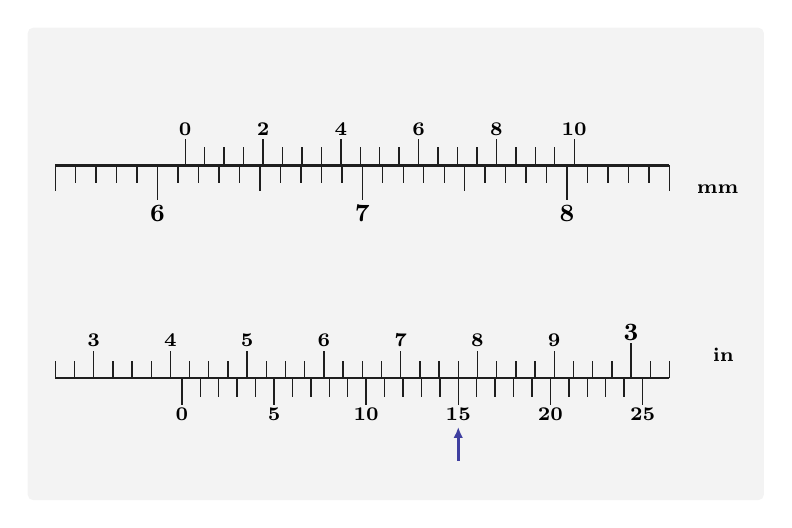
\begin{tikzpicture}[scale=1]
  \fill[figpanel,rounded corners=2pt] (-0.35,-1.55) rectangle (9,4.45);
  \begin{scope}[yshift=2.70cm]
  \draw[scb] (0,0) -- (7.8,0);
  \draw[sc] (0,0) -- (0,-0.32);
  \draw[sc] (0.26,0) -- (0.26,-0.22);
  \draw[sc] (0.52,0) -- (0.52,-0.22);
  \draw[sc] (0.78,0) -- (0.78,-0.22);
  \draw[sc] (1.04,0) -- (1.04,-0.22);
  \draw[sc] (1.3,0) -- (1.3,-0.44);
  \node[lab,below] at (1.3,-0.46) {6};
  \draw[sc] (1.56,0) -- (1.56,-0.22);
  \draw[sc] (1.82,0) -- (1.82,-0.22);
  \draw[sc] (2.08,0) -- (2.08,-0.22);
  \draw[sc] (2.34,0) -- (2.34,-0.22);
  \draw[sc] (2.6,0) -- (2.6,-0.32);
  \draw[sc] (2.86,0) -- (2.86,-0.22);
  \draw[sc] (3.12,0) -- (3.12,-0.22);
  \draw[sc] (3.38,0) -- (3.38,-0.22);
  \draw[sc] (3.64,0) -- (3.64,-0.22);
  \draw[sc] (3.9,0) -- (3.9,-0.44);
  \node[lab,below] at (3.9,-0.46) {7};
  \draw[sc] (4.16,0) -- (4.16,-0.22);
  \draw[sc] (4.42,0) -- (4.42,-0.22);
  \draw[sc] (4.68,0) -- (4.68,-0.22);
  \draw[sc] (4.94,0) -- (4.94,-0.22);
  \draw[sc] (5.2,0) -- (5.2,-0.32);
  \draw[sc] (5.46,0) -- (5.46,-0.22);
  \draw[sc] (5.72,0) -- (5.72,-0.22);
  \draw[sc] (5.98,0) -- (5.98,-0.22);
  \draw[sc] (6.24,0) -- (6.24,-0.22);
  \draw[sc] (6.5,0) -- (6.5,-0.44);
  \node[lab,below] at (6.5,-0.46) {8};
  \draw[sc] (6.76,0) -- (6.76,-0.22);
  \draw[sc] (7.02,0) -- (7.02,-0.22);
  \draw[sc] (7.28,0) -- (7.28,-0.22);
  \draw[sc] (7.54,0) -- (7.54,-0.22);
  \draw[sc] (7.8,0) -- (7.8,-0.32);
  \draw[sc] (1.651,0) -- (1.651,0.34);
  \node[labs,above] at (1.651,0.34) {0};
  \draw[sc] (1.898,0) -- (1.898,0.24);
  \draw[sc] (2.145,0) -- (2.145,0.24);
  \draw[sc] (2.392,0) -- (2.392,0.24);
  \draw[sc] (2.639,0) -- (2.639,0.34);
  \node[labs,above] at (2.639,0.34) {2};
  \draw[sc] (2.886,0) -- (2.886,0.24);
  \draw[sc] (3.133,0) -- (3.133,0.24);
  \draw[sc] (3.38,0) -- (3.38,0.24);
  \draw[sc] (3.627,0) -- (3.627,0.34);
  \node[labs,above] at (3.627,0.34) {4};
  \draw[sc] (3.874,0) -- (3.874,0.24);
  \draw[sc] (4.121,0) -- (4.121,0.24);
  \draw[sc] (4.368,0) -- (4.368,0.24);
  \draw[sc] (4.615,0) -- (4.615,0.34);
  \node[labs,above] at (4.615,0.34) {6};
  \draw[sc] (4.862,0) -- (4.862,0.24);
  \draw[sc] (5.109,0) -- (5.109,0.24);
  \draw[sc] (5.356,0) -- (5.356,0.24);
  \draw[sc] (5.603,0) -- (5.603,0.34);
  \node[labs,above] at (5.603,0.34) {8};
  \draw[sc] (5.85,0) -- (5.85,0.24);
  \draw[sc] (6.097,0) -- (6.097,0.24);
  \draw[sc] (6.344,0) -- (6.344,0.24);
  \draw[sc] (6.591,0) -- (6.591,0.34);
  \node[labs,above] at (6.591,0.34) {10};
  \node[labs,left] at (8.72,-0.30) {mm};
  \end{scope}
  \begin{scope}[yshift=0cm]
  \draw[scb] (0,0) -- (7.8,0);
  \draw[sc] (0,0) -- (0,0.22);
  \draw[sc] (0.2437,0) -- (0.2437,0.22);
  \draw[sc] (0.4875,0) -- (0.4875,0.34);
  \node[labs,above] at (0.4875,0.36) {3};
  \draw[sc] (0.7313,0) -- (0.7313,0.22);
  \draw[sc] (0.975,0) -- (0.975,0.22);
  \draw[sc] (1.2188,0) -- (1.2188,0.22);
  \draw[sc] (1.4625,0) -- (1.4625,0.34);
  \node[labs,above] at (1.4625,0.36) {4};
  \draw[sc] (1.7063,0) -- (1.7063,0.22);
  \draw[sc] (1.95,0) -- (1.95,0.22);
  \draw[sc] (2.1938,0) -- (2.1938,0.22);
  \draw[sc] (2.4375,0) -- (2.4375,0.34);
  \node[labs,above] at (2.4375,0.36) {5};
  \draw[sc] (2.6813,0) -- (2.6813,0.22);
  \draw[sc] (2.925,0) -- (2.925,0.22);
  \draw[sc] (3.1688,0) -- (3.1688,0.22);
  \draw[sc] (3.4125,0) -- (3.4125,0.34);
  \node[labs,above] at (3.4125,0.36) {6};
  \draw[sc] (3.6562,0) -- (3.6562,0.22);
  \draw[sc] (3.9,0) -- (3.9,0.22);
  \draw[sc] (4.1438,0) -- (4.1438,0.22);
  \draw[sc] (4.3875,0) -- (4.3875,0.34);
  \node[labs,above] at (4.3875,0.36) {7};
  \draw[sc] (4.6313,0) -- (4.6313,0.22);
  \draw[sc] (4.875,0) -- (4.875,0.22);
  \draw[sc] (5.1188,0) -- (5.1188,0.22);
  \draw[sc] (5.3625,0) -- (5.3625,0.34);
  \node[labs,above] at (5.3625,0.36) {8};
  \draw[sc] (5.6063,0) -- (5.6063,0.22);
  \draw[sc] (5.85,0) -- (5.85,0.22);
  \draw[sc] (6.0938,0) -- (6.0938,0.22);
  \draw[sc] (6.3375,0) -- (6.3375,0.34);
  \node[labs,above] at (6.3375,0.36) {9};
  \draw[sc] (6.5813,0) -- (6.5813,0.22);
  \draw[sc] (6.825,0) -- (6.825,0.22);
  \draw[sc] (7.0688,0) -- (7.0688,0.22);
  \draw[sc] (7.3125,0) -- (7.3125,0.44);
  \node[lab,above] at (7.3125,0.44) {3};
  \draw[sc] (7.5563,0) -- (7.5563,0.22);
  \draw[sc] (7.8,0) -- (7.8,0.22);
  \draw[sc] (1.6088,0) -- (1.6088,-0.34);
  \node[labs,below] at (1.6088,-0.34) {0};
  \draw[sc] (1.8428,0) -- (1.8428,-0.24);
  \draw[sc] (2.0768,0) -- (2.0768,-0.24);
  \draw[sc] (2.3108,0) -- (2.3108,-0.24);
  \draw[sc] (2.5448,0) -- (2.5448,-0.24);
  \draw[sc] (2.7788,0) -- (2.7788,-0.34);
  \node[labs,below] at (2.7788,-0.34) {5};
  \draw[sc] (3.0128,0) -- (3.0128,-0.24);
  \draw[sc] (3.2468,0) -- (3.2468,-0.24);
  \draw[sc] (3.4808,0) -- (3.4808,-0.24);
  \draw[sc] (3.7148,0) -- (3.7148,-0.24);
  \draw[sc] (3.9488,0) -- (3.9488,-0.34);
  \node[labs,below] at (3.9488,-0.34) {10};
  \draw[sc] (4.1828,0) -- (4.1828,-0.24);
  \draw[sc] (4.4168,0) -- (4.4168,-0.24);
  \draw[sc] (4.6507,0) -- (4.6507,-0.24);
  \draw[sc] (4.8847,0) -- (4.8847,-0.24);
  \draw[sc] (5.1187,0) -- (5.1187,-0.34);
  \node[labs,below] at (5.1187,-0.34) {15};
  \draw[sc] (5.3527,0) -- (5.3527,-0.24);
  \draw[sc] (5.5867,0) -- (5.5867,-0.24);
  \draw[sc] (5.8207,0) -- (5.8207,-0.24);
  \draw[sc] (6.0548,0) -- (6.0548,-0.24);
  \draw[sc] (6.2888,0) -- (6.2888,-0.34);
  \node[labs,below] at (6.2888,-0.34) {20};
  \draw[sc] (6.5228,0) -- (6.5228,-0.24);
  \draw[sc] (6.7568,0) -- (6.7568,-0.24);
  \draw[sc] (6.9908,0) -- (6.9908,-0.24);
  \draw[sc] (7.2248,0) -- (7.2248,-0.24);
  \draw[sc] (7.4588,0) -- (7.4588,-0.34);
  \node[labs,below] at (7.4588,-0.34) {25};
  \draw[ptr] (5.1187,-1.05) -- (5.1187,-0.62);
  \node[labs,left] at (8.66,0.30) {in};
  \end{scope}
\end{tikzpicture}
}

\newcommand{\figQBC}{%
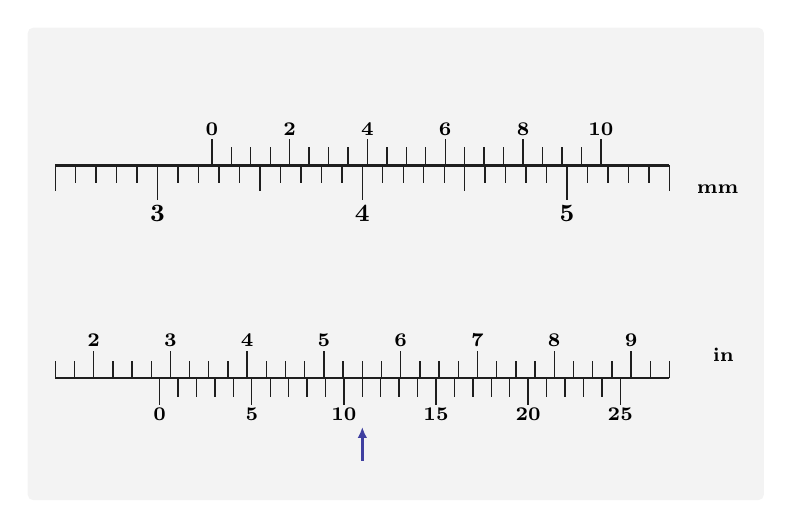
\begin{tikzpicture}[scale=1]
  \fill[figpanel,rounded corners=2pt] (-0.35,-1.55) rectangle (9,4.45);
  \begin{scope}[yshift=2.70cm]
  \draw[scb] (0,0) -- (7.8,0);
  \draw[sc] (0,0) -- (0,-0.32);
  \draw[sc] (0.26,0) -- (0.26,-0.22);
  \draw[sc] (0.52,0) -- (0.52,-0.22);
  \draw[sc] (0.78,0) -- (0.78,-0.22);
  \draw[sc] (1.04,0) -- (1.04,-0.22);
  \draw[sc] (1.3,0) -- (1.3,-0.44);
  \node[lab,below] at (1.3,-0.46) {3};
  \draw[sc] (1.56,0) -- (1.56,-0.22);
  \draw[sc] (1.82,0) -- (1.82,-0.22);
  \draw[sc] (2.08,0) -- (2.08,-0.22);
  \draw[sc] (2.34,0) -- (2.34,-0.22);
  \draw[sc] (2.6,0) -- (2.6,-0.32);
  \draw[sc] (2.86,0) -- (2.86,-0.22);
  \draw[sc] (3.12,0) -- (3.12,-0.22);
  \draw[sc] (3.38,0) -- (3.38,-0.22);
  \draw[sc] (3.64,0) -- (3.64,-0.22);
  \draw[sc] (3.9,0) -- (3.9,-0.44);
  \node[lab,below] at (3.9,-0.46) {4};
  \draw[sc] (4.16,0) -- (4.16,-0.22);
  \draw[sc] (4.42,0) -- (4.42,-0.22);
  \draw[sc] (4.68,0) -- (4.68,-0.22);
  \draw[sc] (4.94,0) -- (4.94,-0.22);
  \draw[sc] (5.2,0) -- (5.2,-0.32);
  \draw[sc] (5.46,0) -- (5.46,-0.22);
  \draw[sc] (5.72,0) -- (5.72,-0.22);
  \draw[sc] (5.98,0) -- (5.98,-0.22);
  \draw[sc] (6.24,0) -- (6.24,-0.22);
  \draw[sc] (6.5,0) -- (6.5,-0.44);
  \node[lab,below] at (6.5,-0.46) {5};
  \draw[sc] (6.76,0) -- (6.76,-0.22);
  \draw[sc] (7.02,0) -- (7.02,-0.22);
  \draw[sc] (7.28,0) -- (7.28,-0.22);
  \draw[sc] (7.54,0) -- (7.54,-0.22);
  \draw[sc] (7.8,0) -- (7.8,-0.32);
  \draw[sc] (1.989,0) -- (1.989,0.34);
  \node[labs,above] at (1.989,0.34) {0};
  \draw[sc] (2.236,0) -- (2.236,0.24);
  \draw[sc] (2.483,0) -- (2.483,0.24);
  \draw[sc] (2.73,0) -- (2.73,0.24);
  \draw[sc] (2.977,0) -- (2.977,0.34);
  \node[labs,above] at (2.977,0.34) {2};
  \draw[sc] (3.224,0) -- (3.224,0.24);
  \draw[sc] (3.471,0) -- (3.471,0.24);
  \draw[sc] (3.718,0) -- (3.718,0.24);
  \draw[sc] (3.965,0) -- (3.965,0.34);
  \node[labs,above] at (3.965,0.34) {4};
  \draw[sc] (4.212,0) -- (4.212,0.24);
  \draw[sc] (4.459,0) -- (4.459,0.24);
  \draw[sc] (4.706,0) -- (4.706,0.24);
  \draw[sc] (4.953,0) -- (4.953,0.34);
  \node[labs,above] at (4.953,0.34) {6};
  \draw[sc] (5.2,0) -- (5.2,0.24);
  \draw[sc] (5.447,0) -- (5.447,0.24);
  \draw[sc] (5.694,0) -- (5.694,0.24);
  \draw[sc] (5.941,0) -- (5.941,0.34);
  \node[labs,above] at (5.941,0.34) {8};
  \draw[sc] (6.188,0) -- (6.188,0.24);
  \draw[sc] (6.435,0) -- (6.435,0.24);
  \draw[sc] (6.682,0) -- (6.682,0.24);
  \draw[sc] (6.929,0) -- (6.929,0.34);
  \node[labs,above] at (6.929,0.34) {10};
  \node[labs,left] at (8.72,-0.30) {mm};
  \end{scope}
  \begin{scope}[yshift=0cm]
  \draw[scb] (0,0) -- (7.8,0);
  \draw[sc] (0,0) -- (0,0.22);
  \draw[sc] (0.2438,0) -- (0.2438,0.22);
  \draw[sc] (0.4875,0) -- (0.4875,0.34);
  \node[labs,above] at (0.4875,0.36) {2};
  \draw[sc] (0.7313,0) -- (0.7313,0.22);
  \draw[sc] (0.975,0) -- (0.975,0.22);
  \draw[sc] (1.2188,0) -- (1.2188,0.22);
  \draw[sc] (1.4625,0) -- (1.4625,0.34);
  \node[labs,above] at (1.4625,0.36) {3};
  \draw[sc] (1.7063,0) -- (1.7063,0.22);
  \draw[sc] (1.95,0) -- (1.95,0.22);
  \draw[sc] (2.1938,0) -- (2.1938,0.22);
  \draw[sc] (2.4375,0) -- (2.4375,0.34);
  \node[labs,above] at (2.4375,0.36) {4};
  \draw[sc] (2.6813,0) -- (2.6813,0.22);
  \draw[sc] (2.925,0) -- (2.925,0.22);
  \draw[sc] (3.1688,0) -- (3.1688,0.22);
  \draw[sc] (3.4125,0) -- (3.4125,0.34);
  \node[labs,above] at (3.4125,0.36) {5};
  \draw[sc] (3.6563,0) -- (3.6563,0.22);
  \draw[sc] (3.9,0) -- (3.9,0.22);
  \draw[sc] (4.1438,0) -- (4.1438,0.22);
  \draw[sc] (4.3875,0) -- (4.3875,0.34);
  \node[labs,above] at (4.3875,0.36) {6};
  \draw[sc] (4.6313,0) -- (4.6313,0.22);
  \draw[sc] (4.875,0) -- (4.875,0.22);
  \draw[sc] (5.1188,0) -- (5.1188,0.22);
  \draw[sc] (5.3625,0) -- (5.3625,0.34);
  \node[labs,above] at (5.3625,0.36) {7};
  \draw[sc] (5.6063,0) -- (5.6063,0.22);
  \draw[sc] (5.85,0) -- (5.85,0.22);
  \draw[sc] (6.0938,0) -- (6.0938,0.22);
  \draw[sc] (6.3375,0) -- (6.3375,0.34);
  \node[labs,above] at (6.3375,0.36) {8};
  \draw[sc] (6.5813,0) -- (6.5813,0.22);
  \draw[sc] (6.825,0) -- (6.825,0.22);
  \draw[sc] (7.0688,0) -- (7.0688,0.22);
  \draw[sc] (7.3125,0) -- (7.3125,0.34);
  \node[labs,above] at (7.3125,0.36) {9};
  \draw[sc] (7.5563,0) -- (7.5563,0.22);
  \draw[sc] (7.8,0) -- (7.8,0.22);
  \draw[sc] (1.326,0) -- (1.326,-0.34);
  \node[labs,below] at (1.326,-0.34) {0};
  \draw[sc] (1.56,0) -- (1.56,-0.24);
  \draw[sc] (1.794,0) -- (1.794,-0.24);
  \draw[sc] (2.028,0) -- (2.028,-0.24);
  \draw[sc] (2.262,0) -- (2.262,-0.24);
  \draw[sc] (2.496,0) -- (2.496,-0.34);
  \node[labs,below] at (2.496,-0.34) {5};
  \draw[sc] (2.73,0) -- (2.73,-0.24);
  \draw[sc] (2.964,0) -- (2.964,-0.24);
  \draw[sc] (3.198,0) -- (3.198,-0.24);
  \draw[sc] (3.432,0) -- (3.432,-0.24);
  \draw[sc] (3.666,0) -- (3.666,-0.34);
  \node[labs,below] at (3.666,-0.34) {10};
  \draw[sc] (3.9,0) -- (3.9,-0.24);
  \draw[sc] (4.134,0) -- (4.134,-0.24);
  \draw[sc] (4.368,0) -- (4.368,-0.24);
  \draw[sc] (4.602,0) -- (4.602,-0.24);
  \draw[sc] (4.836,0) -- (4.836,-0.34);
  \node[labs,below] at (4.836,-0.34) {15};
  \draw[sc] (5.07,0) -- (5.07,-0.24);
  \draw[sc] (5.304,0) -- (5.304,-0.24);
  \draw[sc] (5.538,0) -- (5.538,-0.24);
  \draw[sc] (5.772,0) -- (5.772,-0.24);
  \draw[sc] (6.006,0) -- (6.006,-0.34);
  \node[labs,below] at (6.006,-0.34) {20};
  \draw[sc] (6.24,0) -- (6.24,-0.24);
  \draw[sc] (6.474,0) -- (6.474,-0.24);
  \draw[sc] (6.708,0) -- (6.708,-0.24);
  \draw[sc] (6.942,0) -- (6.942,-0.24);
  \draw[sc] (7.176,0) -- (7.176,-0.34);
  \node[labs,below] at (7.176,-0.34) {25};
  \draw[ptr] (3.9,-1.05) -- (3.9,-0.62);
  \node[labs,left] at (8.66,0.30) {in};
  \end{scope}
\end{tikzpicture}
}

\newcommand{\figQBF}{%
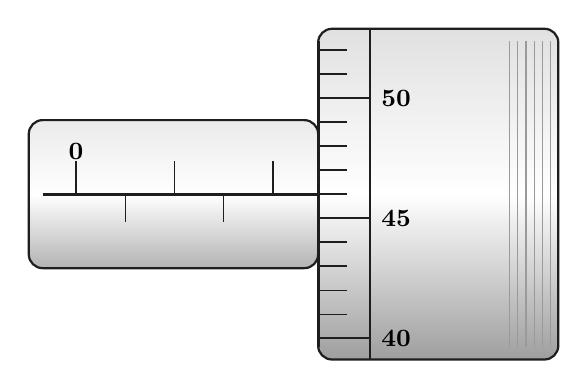
\begin{tikzpicture}[scale=1]
  \shade[rounded corners=5pt,top color=black!8,bottom color=black!30,middle color=white] (0,-0.94) rectangle (3.675,0.94);
  \draw[scb,rounded corners=5pt] (0,-0.94) rectangle (3.675,0.94);
  \draw[draw=figline,line width=1.1pt] (0.18,0) -- (3.675,0);
  \draw[sc] (0.6,0) -- (0.6,0.42);
  \node[lab,above] at (0.6,0.40) {0};
  \draw[sc] (1.225,0) -- (1.225,-0.36);
  \draw[sc] (1.85,0) -- (1.85,0.42);
  \draw[sc] (2.475,0) -- (2.475,-0.36);
  \draw[sc] (3.1,0) -- (3.1,0.42);
  \shade[rounded corners=5pt,top color=black!12,bottom color=black!38,middle color=white] (3.675,-2.1) rectangle (6.725,2.1);
  \draw[scb,rounded corners=5pt] (3.675,-2.1) rectangle (6.725,2.1);
  \draw[draw=figline,line width=1.0pt] (3.675,-1.94) -- (3.675,1.94);
  \draw[sc] (4.335,-2.1) -- (4.335,2.1);
  \draw[draw=figline!45,line width=0.4pt] (6.105,-1.94) -- (6.105,1.94);
  \draw[draw=figline!45,line width=0.4pt] (6.21,-1.94) -- (6.21,1.94);
  \draw[draw=figline!45,line width=0.4pt] (6.315,-1.94) -- (6.315,1.94);
  \draw[draw=figline!45,line width=0.4pt] (6.42,-1.94) -- (6.42,1.94);
  \draw[draw=figline!45,line width=0.4pt] (6.525,-1.94) -- (6.525,1.94);
  \draw[draw=figline!45,line width=0.4pt] (6.63,-1.94) -- (6.63,1.94);
  \draw[draw=figline,line width=0.9pt] (3.675,-1.83) -- (4.335,-1.83);
  \node[lab,right] at (4.435,-1.83) {40};
  \draw[draw=figline,line width=0.5pt] (3.675,-1.525) -- (4.038,-1.525);
  \draw[draw=figline,line width=0.5pt] (3.675,-1.22) -- (4.038,-1.22);
  \draw[draw=figline,line width=0.5pt] (3.675,-0.915) -- (4.038,-0.915);
  \draw[draw=figline,line width=0.5pt] (3.675,-0.61) -- (4.038,-0.61);
  \draw[draw=figline,line width=0.9pt] (3.675,-0.305) -- (4.335,-0.305);
  \node[lab,right] at (4.435,-0.305) {45};
  \draw[draw=figline,line width=0.5pt] (3.675,0) -- (4.038,0);
  \draw[draw=figline,line width=0.5pt] (3.675,0.305) -- (4.038,0.305);
  \draw[draw=figline,line width=0.5pt] (3.675,0.61) -- (4.038,0.61);
  \draw[draw=figline,line width=0.5pt] (3.675,0.915) -- (4.038,0.915);
  \draw[draw=figline,line width=0.9pt] (3.675,1.22) -- (4.335,1.22);
  \node[lab,right] at (4.435,1.22) {50};
  \draw[draw=figline,line width=0.5pt] (3.675,1.525) -- (4.038,1.525);
  \draw[draw=figline,line width=0.5pt] (3.675,1.83) -- (4.038,1.83);
\end{tikzpicture}
}

\newcommand{\figQBG}{%
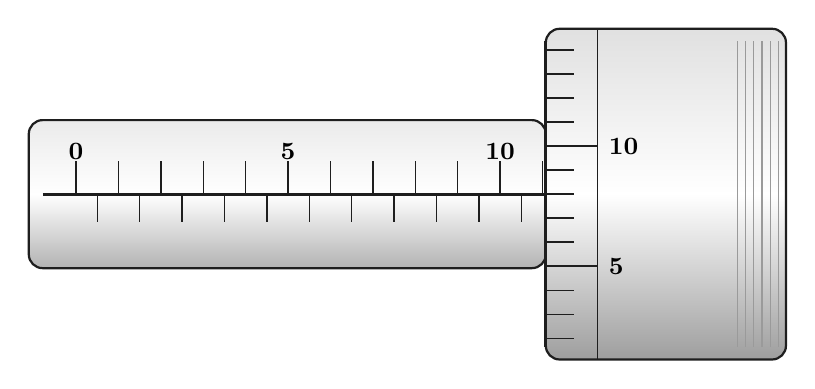
\begin{tikzpicture}[scale=1]
  \shade[rounded corners=5pt,top color=black!8,bottom color=black!30,middle color=white] (0,-0.94) rectangle (6.5662,0.94);
  \draw[scb,rounded corners=5pt] (0,-0.94) rectangle (6.5662,0.94);
  \draw[draw=figline,line width=1.1pt] (0.18,0) -- (6.5662,0);
  \draw[sc] (0.6,0) -- (0.6,0.42);
  \node[lab,above] at (0.6,0.40) {0};
  \draw[sc] (0.8692,0) -- (0.8692,-0.36);
  \draw[sc] (1.1385,0) -- (1.1385,0.42);
  \draw[sc] (1.4077,0) -- (1.4077,-0.36);
  \draw[sc] (1.6769,0) -- (1.6769,0.42);
  \draw[sc] (1.9462,0) -- (1.9462,-0.36);
  \draw[sc] (2.2154,0) -- (2.2154,0.42);
  \draw[sc] (2.4846,0) -- (2.4846,-0.36);
  \draw[sc] (2.7538,0) -- (2.7538,0.42);
  \draw[sc] (3.0231,0) -- (3.0231,-0.36);
  \draw[sc] (3.2923,0) -- (3.2923,0.42);
  \node[lab,above] at (3.2923,0.40) {5};
  \draw[sc] (3.5615,0) -- (3.5615,-0.36);
  \draw[sc] (3.8308,0) -- (3.8308,0.42);
  \draw[sc] (4.1,0) -- (4.1,-0.36);
  \draw[sc] (4.3692,0) -- (4.3692,0.42);
  \draw[sc] (4.6385,0) -- (4.6385,-0.36);
  \draw[sc] (4.9077,0) -- (4.9077,0.42);
  \draw[sc] (5.1769,0) -- (5.1769,-0.36);
  \draw[sc] (5.4462,0) -- (5.4462,0.42);
  \draw[sc] (5.7154,0) -- (5.7154,-0.36);
  \draw[sc] (5.9846,0) -- (5.9846,0.42);
  \node[lab,above] at (5.9846,0.40) {10};
  \draw[sc] (6.2538,0) -- (6.2538,-0.36);
  \draw[sc] (6.5231,0) -- (6.5231,0.42);
  \shade[rounded corners=5pt,top color=black!12,bottom color=black!38,middle color=white] (6.5662,-2.1) rectangle (9.6162,2.1);
  \draw[scb,rounded corners=5pt] (6.5662,-2.1) rectangle (9.6162,2.1);
  \draw[draw=figline,line width=1.0pt] (6.5662,-1.94) -- (6.5662,1.94);
  \draw[sc] (7.2262,-2.1) -- (7.2262,2.1);
  \draw[draw=figline!45,line width=0.4pt] (8.9962,-1.94) -- (8.9962,1.94);
  \draw[draw=figline!45,line width=0.4pt] (9.1012,-1.94) -- (9.1012,1.94);
  \draw[draw=figline!45,line width=0.4pt] (9.2062,-1.94) -- (9.2062,1.94);
  \draw[draw=figline!45,line width=0.4pt] (9.3112,-1.94) -- (9.3112,1.94);
  \draw[draw=figline!45,line width=0.4pt] (9.4162,-1.94) -- (9.4162,1.94);
  \draw[draw=figline!45,line width=0.4pt] (9.5212,-1.94) -- (9.5212,1.94);
  \draw[draw=figline,line width=0.5pt] (6.5662,-1.83) -- (6.9292,-1.83);
  \draw[draw=figline,line width=0.5pt] (6.5662,-1.525) -- (6.9292,-1.525);
  \draw[draw=figline,line width=0.5pt] (6.5662,-1.22) -- (6.9292,-1.22);
  \draw[draw=figline,line width=0.9pt] (6.5662,-0.915) -- (7.2262,-0.915);
  \node[lab,right] at (7.3262,-0.915) {5};
  \draw[draw=figline,line width=0.5pt] (6.5662,-0.61) -- (6.9292,-0.61);
  \draw[draw=figline,line width=0.5pt] (6.5662,-0.305) -- (6.9292,-0.305);
  \draw[draw=figline,line width=0.5pt] (6.5662,0) -- (6.9292,0);
  \draw[draw=figline,line width=0.5pt] (6.5662,0.305) -- (6.9292,0.305);
  \draw[draw=figline,line width=0.9pt] (6.5662,0.61) -- (7.2262,0.61);
  \node[lab,right] at (7.3262,0.61) {10};
  \draw[draw=figline,line width=0.5pt] (6.5662,0.915) -- (6.9292,0.915);
  \draw[draw=figline,line width=0.5pt] (6.5662,1.22) -- (6.9292,1.22);
  \draw[draw=figline,line width=0.5pt] (6.5662,1.525) -- (6.9292,1.525);
  \draw[draw=figline,line width=0.5pt] (6.5662,1.83) -- (6.9292,1.83);
\end{tikzpicture}
}

\newcommand{\figQBH}{%
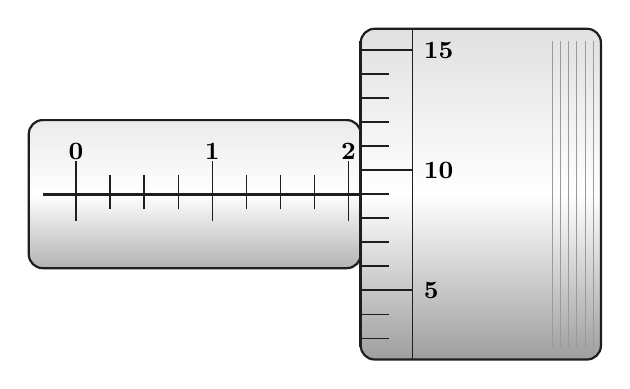
\begin{tikzpicture}[scale=1]
  \shade[rounded corners=5pt,top color=black!8,bottom color=black!30,middle color=white] (0,-0.94) rectangle (4.2159,0.94);
  \draw[scb,rounded corners=5pt] (0,-0.94) rectangle (4.2159,0.94);
  \draw[draw=figline,line width=1.1pt] (0.18,0) -- (4.2159,0);
  \draw[sc] (0.6,-0.336) -- (0.6,0.42);
  \node[lab,above] at (0.6,0.40) {0};
  \draw[sc] (1.0325,-0.192) -- (1.0325,0.24);
  \draw[sc] (1.4651,-0.192) -- (1.4651,0.24);
  \draw[sc] (1.8976,-0.192) -- (1.8976,0.24);
  \draw[sc] (2.3301,-0.336) -- (2.3301,0.42);
  \node[lab,above] at (2.3301,0.40) {1};
  \draw[sc] (2.7626,-0.192) -- (2.7626,0.24);
  \draw[sc] (3.1952,-0.192) -- (3.1952,0.24);
  \draw[sc] (3.6277,-0.192) -- (3.6277,0.24);
  \draw[sc] (4.0602,-0.336) -- (4.0602,0.42);
  \node[lab,above] at (4.0602,0.40) {2};
  \shade[rounded corners=5pt,top color=black!12,bottom color=black!38,middle color=white] (4.2159,-2.1) rectangle (7.2659,2.1);
  \draw[scb,rounded corners=5pt] (4.2159,-2.1) rectangle (7.2659,2.1);
  \draw[draw=figline,line width=1.0pt] (4.2159,-1.94) -- (4.2159,1.94);
  \draw[sc] (4.8759,-2.1) -- (4.8759,2.1);
  \draw[draw=figline!45,line width=0.4pt] (6.6459,-1.94) -- (6.6459,1.94);
  \draw[draw=figline!45,line width=0.4pt] (6.7509,-1.94) -- (6.7509,1.94);
  \draw[draw=figline!45,line width=0.4pt] (6.8559,-1.94) -- (6.8559,1.94);
  \draw[draw=figline!45,line width=0.4pt] (6.9609,-1.94) -- (6.9609,1.94);
  \draw[draw=figline!45,line width=0.4pt] (7.0659,-1.94) -- (7.0659,1.94);
  \draw[draw=figline!45,line width=0.4pt] (7.1709,-1.94) -- (7.1709,1.94);
  \draw[draw=figline,line width=0.5pt] (4.2159,-1.83) -- (4.5789,-1.83);
  \draw[draw=figline,line width=0.5pt] (4.2159,-1.525) -- (4.5789,-1.525);
  \draw[draw=figline,line width=0.9pt] (4.2159,-1.22) -- (4.8759,-1.22);
  \node[lab,right] at (4.9759,-1.22) {5};
  \draw[draw=figline,line width=0.5pt] (4.2159,-0.915) -- (4.5789,-0.915);
  \draw[draw=figline,line width=0.5pt] (4.2159,-0.61) -- (4.5789,-0.61);
  \draw[draw=figline,line width=0.5pt] (4.2159,-0.305) -- (4.5789,-0.305);
  \draw[draw=figline,line width=0.5pt] (4.2159,0) -- (4.5789,0);
  \draw[draw=figline,line width=0.9pt] (4.2159,0.305) -- (4.8759,0.305);
  \node[lab,right] at (4.9759,0.305) {10};
  \draw[draw=figline,line width=0.5pt] (4.2159,0.61) -- (4.5789,0.61);
  \draw[draw=figline,line width=0.5pt] (4.2159,0.915) -- (4.5789,0.915);
  \draw[draw=figline,line width=0.5pt] (4.2159,1.22) -- (4.5789,1.22);
  \draw[draw=figline,line width=0.5pt] (4.2159,1.525) -- (4.5789,1.525);
  \draw[draw=figline,line width=0.9pt] (4.2159,1.83) -- (4.8759,1.83);
  \node[lab,right] at (4.9759,1.83) {15};
\end{tikzpicture}
}

\newcommand{\figQBI}{%
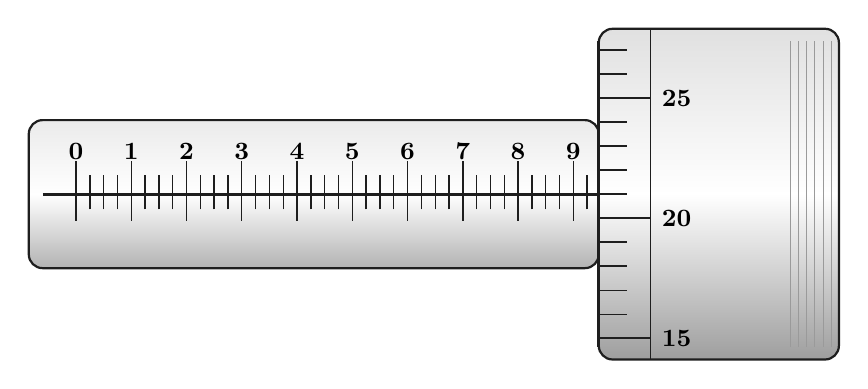
\begin{tikzpicture}[scale=1]
  \shade[rounded corners=5pt,top color=black!8,bottom color=black!30,middle color=white] (0,-0.94) rectangle (7.2386,0.94);
  \draw[scb,rounded corners=5pt] (0,-0.94) rectangle (7.2386,0.94);
  \draw[draw=figline,line width=1.1pt] (0.18,0) -- (7.2386,0);
  \draw[sc] (0.6,-0.336) -- (0.6,0.42);
  \node[lab,above] at (0.6,0.40) {0};
  \draw[sc] (0.7754,-0.192) -- (0.7754,0.24);
  \draw[sc] (0.9509,-0.192) -- (0.9509,0.24);
  \draw[sc] (1.1263,-0.192) -- (1.1263,0.24);
  \draw[sc] (1.3018,-0.336) -- (1.3018,0.42);
  \node[lab,above] at (1.3018,0.40) {1};
  \draw[sc] (1.4772,-0.192) -- (1.4772,0.24);
  \draw[sc] (1.6526,-0.192) -- (1.6526,0.24);
  \draw[sc] (1.8281,-0.192) -- (1.8281,0.24);
  \draw[sc] (2.0035,-0.336) -- (2.0035,0.42);
  \node[lab,above] at (2.0035,0.40) {2};
  \draw[sc] (2.1789,-0.192) -- (2.1789,0.24);
  \draw[sc] (2.3544,-0.192) -- (2.3544,0.24);
  \draw[sc] (2.5298,-0.192) -- (2.5298,0.24);
  \draw[sc] (2.7053,-0.336) -- (2.7053,0.42);
  \node[lab,above] at (2.7053,0.40) {3};
  \draw[sc] (2.8807,-0.192) -- (2.8807,0.24);
  \draw[sc] (3.0561,-0.192) -- (3.0561,0.24);
  \draw[sc] (3.2316,-0.192) -- (3.2316,0.24);
  \draw[sc] (3.407,-0.336) -- (3.407,0.42);
  \node[lab,above] at (3.407,0.40) {4};
  \draw[sc] (3.5825,-0.192) -- (3.5825,0.24);
  \draw[sc] (3.7579,-0.192) -- (3.7579,0.24);
  \draw[sc] (3.9333,-0.192) -- (3.9333,0.24);
  \draw[sc] (4.1088,-0.336) -- (4.1088,0.42);
  \node[lab,above] at (4.1088,0.40) {5};
  \draw[sc] (4.2842,-0.192) -- (4.2842,0.24);
  \draw[sc] (4.4596,-0.192) -- (4.4596,0.24);
  \draw[sc] (4.6351,-0.192) -- (4.6351,0.24);
  \draw[sc] (4.8105,-0.336) -- (4.8105,0.42);
  \node[lab,above] at (4.8105,0.40) {6};
  \draw[sc] (4.986,-0.192) -- (4.986,0.24);
  \draw[sc] (5.1614,-0.192) -- (5.1614,0.24);
  \draw[sc] (5.3368,-0.192) -- (5.3368,0.24);
  \draw[sc] (5.5123,-0.336) -- (5.5123,0.42);
  \node[lab,above] at (5.5123,0.40) {7};
  \draw[sc] (5.6877,-0.192) -- (5.6877,0.24);
  \draw[sc] (5.8632,-0.192) -- (5.8632,0.24);
  \draw[sc] (6.0386,-0.192) -- (6.0386,0.24);
  \draw[sc] (6.214,-0.336) -- (6.214,0.42);
  \node[lab,above] at (6.214,0.40) {8};
  \draw[sc] (6.3895,-0.192) -- (6.3895,0.24);
  \draw[sc] (6.5649,-0.192) -- (6.5649,0.24);
  \draw[sc] (6.7404,-0.192) -- (6.7404,0.24);
  \draw[sc] (6.9158,-0.336) -- (6.9158,0.42);
  \node[lab,above] at (6.9158,0.40) {9};
  \draw[sc] (7.0912,-0.192) -- (7.0912,0.24);
  \shade[rounded corners=5pt,top color=black!12,bottom color=black!38,middle color=white] (7.2386,-2.1) rectangle (10.2886,2.1);
  \draw[scb,rounded corners=5pt] (7.2386,-2.1) rectangle (10.2886,2.1);
  \draw[draw=figline,line width=1.0pt] (7.2386,-1.94) -- (7.2386,1.94);
  \draw[sc] (7.8986,-2.1) -- (7.8986,2.1);
  \draw[draw=figline!45,line width=0.4pt] (9.6686,-1.94) -- (9.6686,1.94);
  \draw[draw=figline!45,line width=0.4pt] (9.7736,-1.94) -- (9.7736,1.94);
  \draw[draw=figline!45,line width=0.4pt] (9.8786,-1.94) -- (9.8786,1.94);
  \draw[draw=figline!45,line width=0.4pt] (9.9836,-1.94) -- (9.9836,1.94);
  \draw[draw=figline!45,line width=0.4pt] (10.0886,-1.94) -- (10.0886,1.94);
  \draw[draw=figline!45,line width=0.4pt] (10.1936,-1.94) -- (10.1936,1.94);
  \draw[draw=figline,line width=0.9pt] (7.2386,-1.83) -- (7.8986,-1.83);
  \node[lab,right] at (7.9986,-1.83) {15};
  \draw[draw=figline,line width=0.5pt] (7.2386,-1.525) -- (7.6016,-1.525);
  \draw[draw=figline,line width=0.5pt] (7.2386,-1.22) -- (7.6016,-1.22);
  \draw[draw=figline,line width=0.5pt] (7.2386,-0.915) -- (7.6016,-0.915);
  \draw[draw=figline,line width=0.5pt] (7.2386,-0.61) -- (7.6016,-0.61);
  \draw[draw=figline,line width=0.9pt] (7.2386,-0.305) -- (7.8986,-0.305);
  \node[lab,right] at (7.9986,-0.305) {20};
  \draw[draw=figline,line width=0.5pt] (7.2386,0) -- (7.6016,0);
  \draw[draw=figline,line width=0.5pt] (7.2386,0.305) -- (7.6016,0.305);
  \draw[draw=figline,line width=0.5pt] (7.2386,0.61) -- (7.6016,0.61);
  \draw[draw=figline,line width=0.5pt] (7.2386,0.915) -- (7.6016,0.915);
  \draw[draw=figline,line width=0.9pt] (7.2386,1.22) -- (7.8986,1.22);
  \node[lab,right] at (7.9986,1.22) {25};
  \draw[draw=figline,line width=0.5pt] (7.2386,1.525) -- (7.6016,1.525);
  \draw[draw=figline,line width=0.5pt] (7.2386,1.83) -- (7.6016,1.83);
\end{tikzpicture}
}


\begin{document}

\begin{center}
  {\LARGE\bfseries EnergyTech}\\[2pt]
  {\Large Chapter 04 --- Version D}\\[6pt]
  Name: \rule{4.5cm}{0.4pt}\quad Group: \rule{3cm}{0.4pt}\quad SPSP ID: \rule{3.5cm}{0.4pt}
\end{center}

\begin{multicols}{2}
\raggedcolumns
% ---------------- Q1 ----------------
\begin{Qbox}{1}{4-1.1}
Determine the accuracy of the measurement; that is, give the number of significant digits for the measurement.\par\medskip $1{,}240{,}000$ lb
\begin{choices}
  \item 3
  \item 4
  \item 7
  \item 2
\end{choices}
\qrcode[height=2.2cm,hyperlink]{https://www.youtube.com/watch?v=FhLOHZ4jlP8}
\end{Qbox}

% ---------------- Q2 ----------------
\begin{Qbox}{2}{4-1.1}
Determine the accuracy of the measurement; that is, give the number of significant digits for the measurement.\par\medskip $918{,}4\overline{0}0$
\begin{choices}
  \item 6
  \item 7
  \item 5
  \item 4
\end{choices}
\qrcode[height=2.2cm,hyperlink]{https://www.youtube.com/watch?v=O2WRBUsIeZc}
\end{Qbox}

% ---------------- Q3 ----------------
\begin{Qbox}{3}{4-1.1}
Determine the accuracy of the measurement; that is, give the number of significant digits for the measurement.\par\medskip $0.000850$ g
\begin{choices}
  \item 4
  \item 2
  \item 7
  \item 3
\end{choices}
\qrcode[height=2.2cm,hyperlink]{https://www.youtube.com/watch?v=29VCgAWuS08}
\end{Qbox}

% ---------------- Q4 ----------------
\begin{Qbox}{4}{4-1.1}
Determine the accuracy of the measurement; that is, give the number of significant digits for the measurement.\par\medskip $0.0374000$ A
\begin{choices}
  \item 7
  \item 8
  \item 6
  \item 5
\end{choices}
\qrcode[height=2.2cm,hyperlink]{https://www.youtube.com/watch?v=gEq2wwiqNB8}
\end{Qbox}

% ---------------- Q5 ----------------
\begin{Qbox}{5}{4-1.1}
Determine the accuracy of the measurement; that is, give the number of significant digits for the measurement.\par\medskip $6{,}013$ m
\begin{choices}
  \item 4
  \item 5
  \item 3
  \item 6
\end{choices}
\qrcode[height=2.2cm,hyperlink]{https://www.youtube.com/watch?v=_FD3dS7Vg3U}
\end{Qbox}

% ---------------- Q6 ----------------
\begin{Qbox}{6}{4-1.1}
Determine the accuracy of the measurement; that is, give the number of significant digits for the measurement.\par\medskip $845{,}700$ g
\begin{choices}
  \item 6
  \item 4
  \item 3
  \item 5
\end{choices}
\qrcode[height=2.2cm,hyperlink]{https://www.youtube.com/watch?v=NZMZXixpuv4}
\end{Qbox}

% ---------------- Q7 ----------------
\begin{Qbox}{7}{4-2.1}
The measurement is 17.40 A. Find the precision.
\begin{choices}
  \item The precision of the measurement is 0.01 A
  \item The precision of the measurement is 0.001 A
  \item The precision of the measurement is 0.1 A
  \item The precision of the measurement is 0.0001 A
\end{choices}
\qrcode[height=2.2cm,hyperlink]{https://www.youtube.com/watch?v=xKxx56lye3g}
\end{Qbox}

% ---------------- Q8 ----------------
\begin{Qbox}{8}{4-2.1}
The measurement is 3.6000 cm. Find the precision.
\begin{choices}
  \item The precision is 0.0001 cm
  \item The precision is 0.000001 cm
  \item The precision is 0.00001 cm
  \item The precision is 0.001 cm
\end{choices}
\qrcode[height=2.2cm,hyperlink]{https://www.youtube.com/watch?v=1JnWFd0IspY}
\end{Qbox}

% ---------------- Q9 ----------------
\begin{Qbox}{9}{4-2.1}
The measurement is 250.0 in. Find the precision.
\begin{choices}
  \item The precision is 1 in
  \item The precision is 0.001 in
  \item The precision is 0.01 in
  \item The precision is 0.1 in
\end{choices}
\qrcode[height=2.2cm,hyperlink]{https://www.youtube.com/watch?v=kZ6FfJt_LTA}
\end{Qbox}

% ---------------- Q10 ----------------
\begin{Qbox}{10}{4-2.1}
The measurement is 947 km. Find the precision.
\begin{choices}
  \item The precision is 1 km
  \item The precision is 0.01 km
  \item The precision is 10 km
  \item The precision is 0.1 km
\end{choices}
\qrcode[height=2.2cm,hyperlink]{https://www.youtube.com/watch?v=Uptz7jfWnVI}
\end{Qbox}

% ---------------- Q11 ----------------
\begin{Qbox}{11}{4-2.1}
The measurement is $21{,}5\overline{0}0$ ft. Find the precision.
\begin{choices}
  \item The precision is 1 ft
  \item The precision is 100 ft
  \item The precision is 0.1 ft
  \item The precision is 10 ft
\end{choices}
\qrcode[height=2.2cm,hyperlink]{https://www.youtube.com/watch?v=SE7YQtbcBeg}
\end{Qbox}

% ---------------- Q12 ----------------
\begin{Qbox}{12}{4-2.1}
The measurement is 60.100 mi. Find the precision.
\begin{choices}
  \item The precision is 0.00001 mi
  \item The precision is 0.0001 mi
  \item The precision is 0.01 mi
  \item The precision is 0.001 mi
\end{choices}
\qrcode[height=2.2cm,hyperlink]{https://www.youtube.com/watch?v=cksn4vK3mhk}
\end{Qbox}

% ---------------- Q13 ----------------
\begin{Qbox}{13}{4-2.2}
The measurement is 3.90600 cm. Find the greatest possible error of the measurement.
\begin{choices}
  \item The greatest possible error is 0.00001 cm
  \item The greatest possible error is 0.000005 cm
  \item The greatest possible error is 0.0000005 cm
  \item The greatest possible error is 0.00005 cm
\end{choices}
\qrcode[height=2.2cm,hyperlink]{https://www.youtube.com/watch?v=L-TsjdvD7ZQ}
\end{Qbox}

% ---------------- Q14 ----------------
\begin{Qbox}{14}{4-2.2}
The measurement is 17.240 m. Find the greatest possible error of the measurement.
\begin{choices}
  \item The greatest possible error is 0.005 m
  \item The greatest possible error is 0.0005 m
  \item The greatest possible error is 0.001 m
  \item The greatest possible error is 0.00005 m
\end{choices}
\qrcode[height=2.2cm,hyperlink]{https://www.youtube.com/watch?v=QKBMWpAA95s}
\end{Qbox}

% ---------------- Q15 ----------------
\begin{Qbox}{15}{4-2.2}
The measurement is 55.10 m. Find the greatest possible error of the measurement.
\begin{choices}
  \item The greatest possible error is 0.005 m
  \item The greatest possible error is 0.0005 m
  \item The greatest possible error is 0.01 m
  \item The greatest possible error is 0.05 m
\end{choices}
\qrcode[height=2.2cm,hyperlink]{https://www.youtube.com/watch?v=7kzsFh5ax-8}
\end{Qbox}

% ---------------- Q16 ----------------
\begin{Qbox}{16}{4-2.1 / 4-2.2}
The measurement is $6\frac{11}{18}$ in. Find the precision and the greatest possible error of the measurement.
\begin{choices}
  \item Precision $=\dfrac{1}{18}$, greatest possible error $=\dfrac{1}{18}$
  \item Precision $=\dfrac{1}{18}$, greatest possible error $=\dfrac{1}{36}$
  \item Precision $=\dfrac{1}{36}$, greatest possible error $=\dfrac{1}{36}$
  \item Precision $=\dfrac{1}{36}$, greatest possible error $=\dfrac{1}{18}$
\end{choices}
\qrcode[height=2.2cm,hyperlink]{https://www.youtube.com/watch?v=FbGULnhUr58}
\end{Qbox}

% ---------------- Q17 ----------------
\begin{Qbox}{17}{4-2.1 / 4-2.2}
The measurement is $14\frac{21}{25}$ in. Find the precision and the greatest possible error of the measurement.
\begin{choices}
  \item Precision $=\dfrac{1}{50}$, greatest possible error $=\dfrac{1}{50}$
  \item Precision $=\dfrac{1}{25}$, greatest possible error $=\dfrac{1}{50}$
  \item Precision $=\dfrac{1}{25}$, greatest possible error $=\dfrac{1}{25}$
  \item Precision $=\dfrac{1}{50}$, greatest possible error $=\dfrac{1}{25}$
\end{choices}
\qrcode[height=2.2cm,hyperlink]{https://www.youtube.com/watch?v=8v8T6GLrV7M}
\end{Qbox}

% ---------------- Q18 ----------------
\begin{Qbox}{18}{4-3.1}
In the given Vernier Caliper, part F is \ldots
\incfig{210}{fig_caliper.png}
\begin{choices}
  \item Beam
  \item Depth gauge
  \item Small jaws
  \item Jaws
\end{choices}
\qrcode[height=2.2cm,hyperlink]{https://www.youtube.com/watch?v=CKAhOUBv_Ck}
\end{Qbox}

% ---------------- Q19 ----------------
\begin{Qbox}{19}{4-3.1}
In the given Vernier Caliper, part H is \ldots
\incfig{210}{fig_caliper.png}
\begin{choices}
  \item Metric Vernier scale
  \item Metric Fixed scale
  \item U.S. Fixed scale
  \item U.S. Vernier scale
\end{choices}
\qrcode[height=2.2cm,hyperlink]{https://www.youtube.com/watch?v=eydw_enMeQk}
\end{Qbox}

% ---------------- Q20 ----------------
\begin{Qbox}{20}{4-3.1}
Read the measurement in millimeter shown on the vernier caliper.
\figbox{\figQBZ}
\begin{choices}
  \item 45.75 mm
  \item 1.801 mm
  \item 45.57 mm
  \item 1.810 mm
\end{choices}
\qrcode[height=2.2cm,hyperlink]{https://www.youtube.com/watch?v=m5Lp71cWcFE}
\end{Qbox}

% ---------------- Q21 ----------------
\begin{Qbox}{21}{4-3.2}
Read the measurement in millimeter shown on the vernier caliper.
\figbox{\figQBA}
\begin{choices}
  \item 103.53 mm
  \item 4.069 mm
  \item 4.096 mm
  \item 103.35 mm
\end{choices}
\qrcode[height=2.2cm,hyperlink]{https://www.youtube.com/watch?v=xVg0hxrQ4Jg}
\end{Qbox}

% ---------------- Q22 ----------------
\begin{Qbox}{22}{4-3.3}
Read the measurement in inch shown on the vernier caliper.
\figbox{\figQBB}
\begin{choices}
  \item 2.415 in
  \item 61.35 in
  \item 0.415 in
  \item 2.451 in
\end{choices}
\qrcode[height=2.2cm,hyperlink]{https://www.youtube.com/watch?v=wcmLZgkqi3M}
\end{Qbox}

% ---------------- Q23 ----------------
\begin{Qbox}{23}{4-3.3}
Read the measurement in inch shown on the vernier caliper.
\figbox{\figQBC}
\begin{choices}
  \item 1.286 in
  \item 32.65 in
  \item 0.286 in
  \item 1.268 in
\end{choices}
\qrcode[height=2.2cm,hyperlink]{https://www.youtube.com/watch?v=bXo3POT01eE}
\end{Qbox}

% ---------------- Q24 ----------------
\begin{Qbox}{24}{4-4.1}
In the given Micrometer Caliper, part J is
\incfig{200}{fig_micrometer.png}
\begin{choices}
  \item Ratchet
  \item Spindle
  \item Anvil
  \item Thimble
\end{choices}
\qrcode[height=2.2cm,hyperlink]{https://www.youtube.com/watch?v=0XkBVkZvfvA}
\end{Qbox}

% ---------------- Q25 ----------------
\begin{Qbox}{25}{4-4.1}
In the given Micrometer Caliper, part G is
\incfig{200}{fig_micrometer.png}
\begin{choices}
  \item Ratchet
  \item Thimble
  \item Anvil
  \item Spindle
\end{choices}
\qrcode[height=2.2cm,hyperlink]{https://www.youtube.com/watch?v=89Bz6HZpME8}
\end{Qbox}

% ---------------- Q26 ----------------
\begin{Qbox}{26}{4-4.2}
Read the measurement shown on the metric micrometer.
\figbox{\figQBF}
\begin{choices}
  \item 2.46 mm
  \item 24.6 mm
  \item 2.45 mm
  \item 2.47 mm
\end{choices}
\qrcode[height=2.2cm,hyperlink]{https://www.youtube.com/watch?v=n0lpdXKX8NA}
\end{Qbox}

% ---------------- Q27 ----------------
\begin{Qbox}{27}{4-4.2}
Read the measurement shown on the metric micrometer.
\figbox{\figQBG}
\begin{choices}
  \item 110.8 mm
  \item 11.07 mm
  \item 11.08 mm
  \item 11.09 mm
\end{choices}
\qrcode[height=2.2cm,hyperlink]{https://www.youtube.com/watch?v=MplthM6FZQU}
\end{Qbox}

% ---------------- Q28 ----------------
\begin{Qbox}{28}{4-4.4}
Read the measurement shown on the U.S. micrometer.
\figbox{\figQBH}
\begin{choices}
  \item 0.200 in
  \item 0.209 in
  \item 2.090 in
  \item 0.234 in
\end{choices}
\qrcode[height=2.2cm,hyperlink]{https://www.youtube.com/watch?v=tTfhEPs7AG4}
\end{Qbox}

% ---------------- Q29 ----------------
\begin{Qbox}{29}{4-4.3}
Read the measurement shown on the U.S. micrometer.
\figbox{\figQBI}
\begin{choices}
  \item 0.925 in
  \item 9.460 in
  \item 0.946 in
  \item 0.971 in
\end{choices}
\qrcode[height=2.2cm,hyperlink]{https://www.youtube.com/watch?v=BSleiTcnV88}
\end{Qbox}

% ---------------- Q30 ----------------
\begin{Qbox}{30}{4-5.1}
Find the measurement that is the most accurate.
\begin{choices}
  \item 2,900 ft
  \item 465 ft
  \item 340 ft
  \item 700 ft
\end{choices}
\qrcode[height=2.2cm,hyperlink]{https://www.youtube.com/watch?v=wFtUtuKgrnI}
\end{Qbox}

% ---------------- Q31 ----------------
\begin{Qbox}{31}{4-5.1}
Find the measurement that is the most accurate.
\begin{choices}
  \item 620 ft
  \item 500 ft
  \item 384 ft
  \item 4,700 ft
\end{choices}
\qrcode[height=2.2cm,hyperlink]{https://www.youtube.com/watch?v=fi2FP7z8XXk}
\end{Qbox}

% ---------------- Q32 ----------------
\begin{Qbox}{32}{4-5.1}
Find the measurement that is the most accurate.
\begin{choices}
  \item 6,300 ft
  \item 857 ft
  \item 490 ft
  \item 200 ft
\end{choices}
\qrcode[height=2.2cm,hyperlink]{https://www.youtube.com/watch?v=S8T8OfIpWdU}
\end{Qbox}

% ---------------- Q33 ----------------
\begin{Qbox}{33}{4-5.1}
Find the measurement that is the most accurate.
\begin{choices}
  \item 5100 ft
  \item 9000 ft
  \item 0.2800 ft
  \item 0.00360 ft
\end{choices}
\qrcode[height=2.2cm,hyperlink]{https://www.youtube.com/watch?v=kmIhRWkySiY}
\end{Qbox}

% ---------------- Q34 ----------------
\begin{Qbox}{34}{4-5.1}
Find the measurement that is the least accurate.
\begin{choices}
  \item 0.000670 in
  \item 2000 in
  \item 48.6000 in
  \item 0.00050 in
\end{choices}
\qrcode[height=2.2cm,hyperlink]{https://www.youtube.com/watch?v=i50ZER16Vic}
\end{Qbox}

% ---------------- Q35 ----------------
\begin{Qbox}{35}{4-5.1}
Find the measurement that is the least accurate.
\begin{choices}
  \item 69300 m
  \item 3160000 m
  \item 580000 m
  \item 0.00840 m
\end{choices}
\qrcode[height=2.2cm,hyperlink]{https://www.youtube.com/watch?v=M7AB8u72_8k}
\end{Qbox}

% ---------------- Q36 ----------------
\begin{Qbox}{36}{4-5.1}
Find the measurement that is the least accurate.
\begin{choices}
  \item 65.0000 in
  \item 0.000370 in
  \item 82000 in
  \item 4000 in
\end{choices}
\qrcode[height=2.2cm,hyperlink]{https://www.youtube.com/watch?v=d32PX6zaUhM}
\end{Qbox}

% ---------------- Q37 ----------------
\begin{Qbox}{37}{4-5.1}
Find the measurement that is the most accurate.
\begin{choices}
  \item 0.0250 A
  \item 0.039 A
  \item 0.038 A
  \item 0.00070 A
\end{choices}
\qrcode[height=2.2cm,hyperlink]{https://www.youtube.com/watch?v=kfDJ24QBcuI}
\end{Qbox}

% ---------------- Q38 ----------------
\begin{Qbox}{38}{4-5.1}
Find the measurement that is the least accurate.
\begin{choices}
  \item 25,000 V
  \item 46,000 V
  \item 7,100,000 V
  \item 30,000 V
\end{choices}
\qrcode[height=2.2cm,hyperlink]{https://www.youtube.com/watch?v=CdvPb7S0h9Y}
\end{Qbox}

% ---------------- Q39 ----------------
\begin{Qbox}{39}{4-5.1}
Find the measurement that is the least accurate.
\begin{choices}
  \item 70,000 V
  \item 3,800,000 V
  \item 92,000 V
  \item 6,400 V
\end{choices}
\qrcode[height=2.2cm,hyperlink]{https://www.youtube.com/watch?v=mdd_74Yj1iA}
\end{Qbox}

% ---------------- Q40 ----------------
\begin{Qbox}{40}{4-5.1}
Find the measurement that is the least accurate.
\begin{choices}
  \item 0.0064 V
  \item 51.00 V
  \item 0.00170 V
  \item 27,300 V
\end{choices}
\qrcode[height=2.2cm,hyperlink]{https://www.youtube.com/watch?v=L0pMHrjqsEg}
\end{Qbox}

% ---------------- Q41 ----------------
\begin{Qbox}{41}{4-5.1}
Find the measurement that is the least accurate.
\begin{choices}
  \item 39,000 ft
  \item 7.10000 ft
  \item 4.910 ft
  \item 0.6700 ft
\end{choices}
\qrcode[height=2.2cm,hyperlink]{https://www.youtube.com/watch?v=nQ0DitEi1Ps}
\end{Qbox}

% ---------------- Q42 ----------------
\begin{Qbox}{42}{4-5.1}
Find the measurement that is the least accurate.
\begin{choices}
  \item 800 ft
  \item 940 ft
  \item 526 ft
  \item 307 ft
\end{choices}
\qrcode[height=2.2cm,hyperlink]{https://www.youtube.com/watch?v=Y1cHxGjrkjU}
\end{Qbox}

% ---------------- Q43 ----------------
\begin{Qbox}{43}{4-5.1}
Find the measurement that is the least accurate.
\begin{choices}
  \item 682 ft
  \item 300 ft
  \item 749 ft
  \item 570 ft
\end{choices}
\qrcode[height=2.2cm,hyperlink]{https://www.youtube.com/watch?v=eBSkNlhA6Wc}
\end{Qbox}

% ---------------- Q44 ----------------
\begin{Qbox}{44}{4-5.1}
Find the measurement that is the least accurate.
\begin{choices}
  \item 900 ft
  \item 380 ft
  \item 241 ft
  \item 209 ft
\end{choices}
\qrcode[height=2.2cm,hyperlink]{https://www.youtube.com/watch?v=toC9PYl0yHk}
\end{Qbox}

% ---------------- Q45 ----------------
\begin{Qbox}{45}{4-5.1}
Use the rules of measurements to evaluate.\par\medskip $(3{,}800\ \text{cm})(46.00\ \text{cm})$
\begin{choices}
  \item 170,000 cm$^2$
  \item 174,800 cm$^2$
  \item 200,000 cm$^2$
  \item 175,000 cm$^2$
\end{choices}
\qrcode[height=2.2cm,hyperlink]{https://www.youtube.com/watch?v=_Xjo5E_pcYo}
\end{Qbox}

% ---------------- Q46 ----------------
\begin{Qbox}{46}{4-6.1}
Use the rules of measurements to evaluate.\par\medskip $(6{,}300\ \text{m})(40\ \text{m})(1810\ \text{m})$
\begin{choices}
  \item 500,000,000 m$^3$
  \item 460,000,000 m$^3$
  \item 456,000,000 m$^3$
  \item 456,100,000 m$^3$
\end{choices}
\qrcode[height=2.2cm,hyperlink]{https://www.youtube.com/watch?v=vd7Sg-5mZc0}
\end{Qbox}

% ---------------- Q47 ----------------
\begin{Qbox}{47}{4-6.1}
Use the rules of measurements to evaluate.\par\medskip $91{,}500$ V $\div\ 4.2$ A
\begin{choices}
  \item 21,800 V/A
  \item 22,000 V/A
  \item 21,786 V/A
  \item 20,000 V/A
\end{choices}
\qrcode[height=2.2cm,hyperlink]{https://www.youtube.com/watch?v=rLAH-4JSDRo}
\end{Qbox}

% ---------------- Q48 ----------------
\begin{Qbox}{48}{4-6.1}
Use the rules of measurements to evaluate.\[ \frac{(5140\ m)(3.2\ L)}{8.0\ s} \]
\begin{choices}
  \item $2{,}056\ mL/s$
  \item $2{,}100\ mL/s$
  \item $2{,}000\ mL/s$
  \item $2.100\ mL/s$
\end{choices}
\qrcode[height=2.2cm,hyperlink]{https://www.youtube.com/watch?v=rGtejzjn64U}
\end{Qbox}

% ---------------- Q49 ----------------
\begin{Qbox}{49}{4-6.1}
Find the area of a rectangle 1.70 cm by 86.0 cm. $(A=l\cdot w)$ (Use the rules for working with measurements).
\begin{choices}
  \item 146.2 cm$^2$
  \item 146 cm$^2$
  \item 100 cm$^2$
  \item 150 cm$^2$
\end{choices}
\qrcode[height=2.2cm,hyperlink]{https://www.youtube.com/watch?v=OVOHkqfkrEI}
\end{Qbox}

% ---------------- Q50 ----------------
\begin{Qbox}{50}{4-6.1}
Find the volume of a rectangular solid when $l=1.90$ ft, $w=7.0$ ft, and $h=53.60$ ft.\par\medskip $V=lwh$, where $l$ length, $w$ width, and $h$ height.\par\medskip (Use the rules for working with measurements)
\begin{choices}
  \item 710 ft$^3$
  \item 713 ft$^3$
  \item 700 ft$^3$
  \item 712.88 ft$^3$
\end{choices}
\qrcode[height=2.2cm,hyperlink]{https://www.youtube.com/watch?v=6P8cDZvSm3M}
\end{Qbox}

\end{multicols}
\end{document}
